
\section{Visualization of Layer Dynamics}

\begin{figure}[h!]
\centering
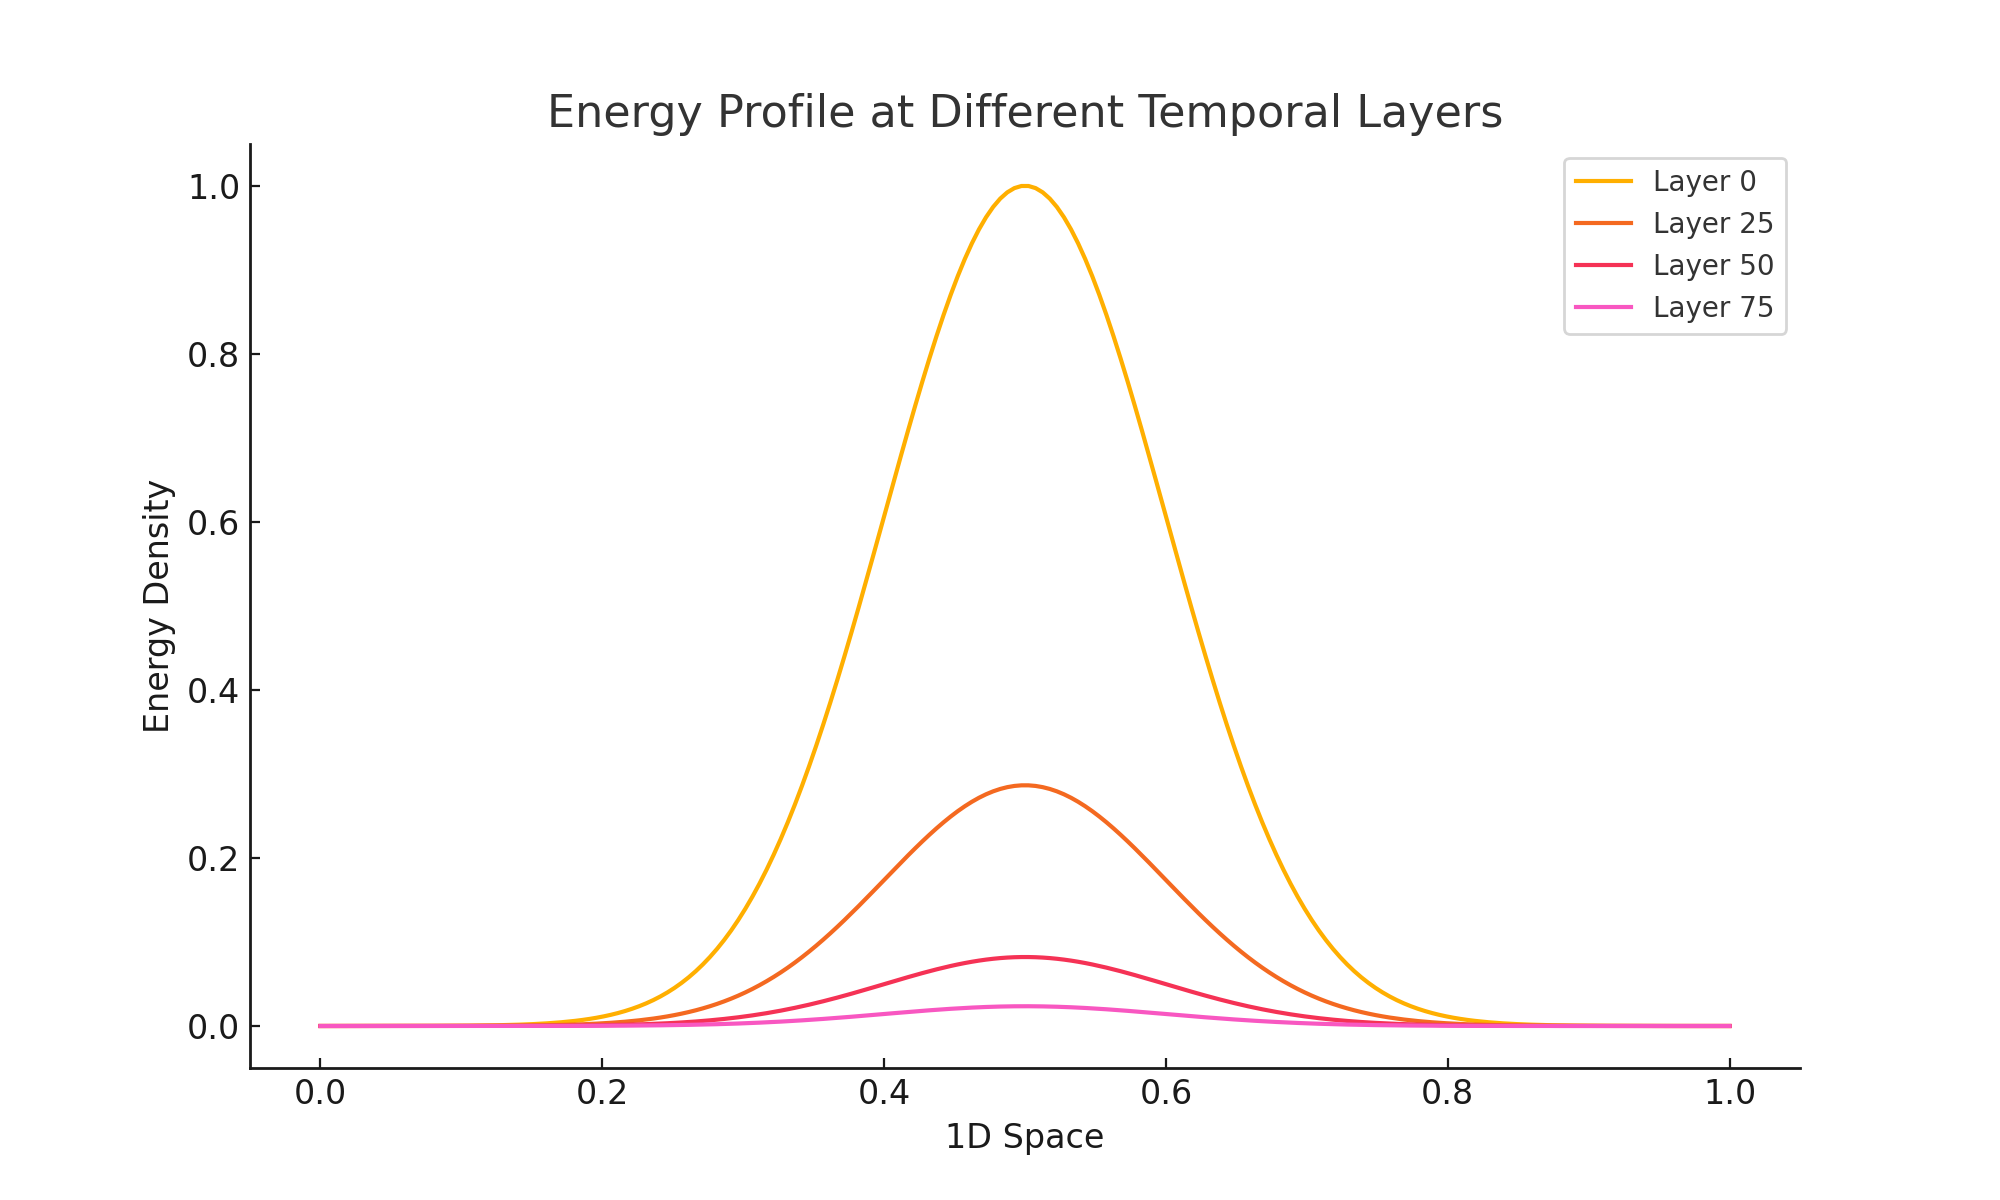
\includegraphics[width=0.9\linewidth]{05_Simulations/energy_profiles.png}
\caption{Energy profiles across temporal layers. Each curve represents the energy density distribution at a given discrete temporal layer.}\label{fig:interactivitystate}
\end{figure}

\begin{figure}[h!]
\centering
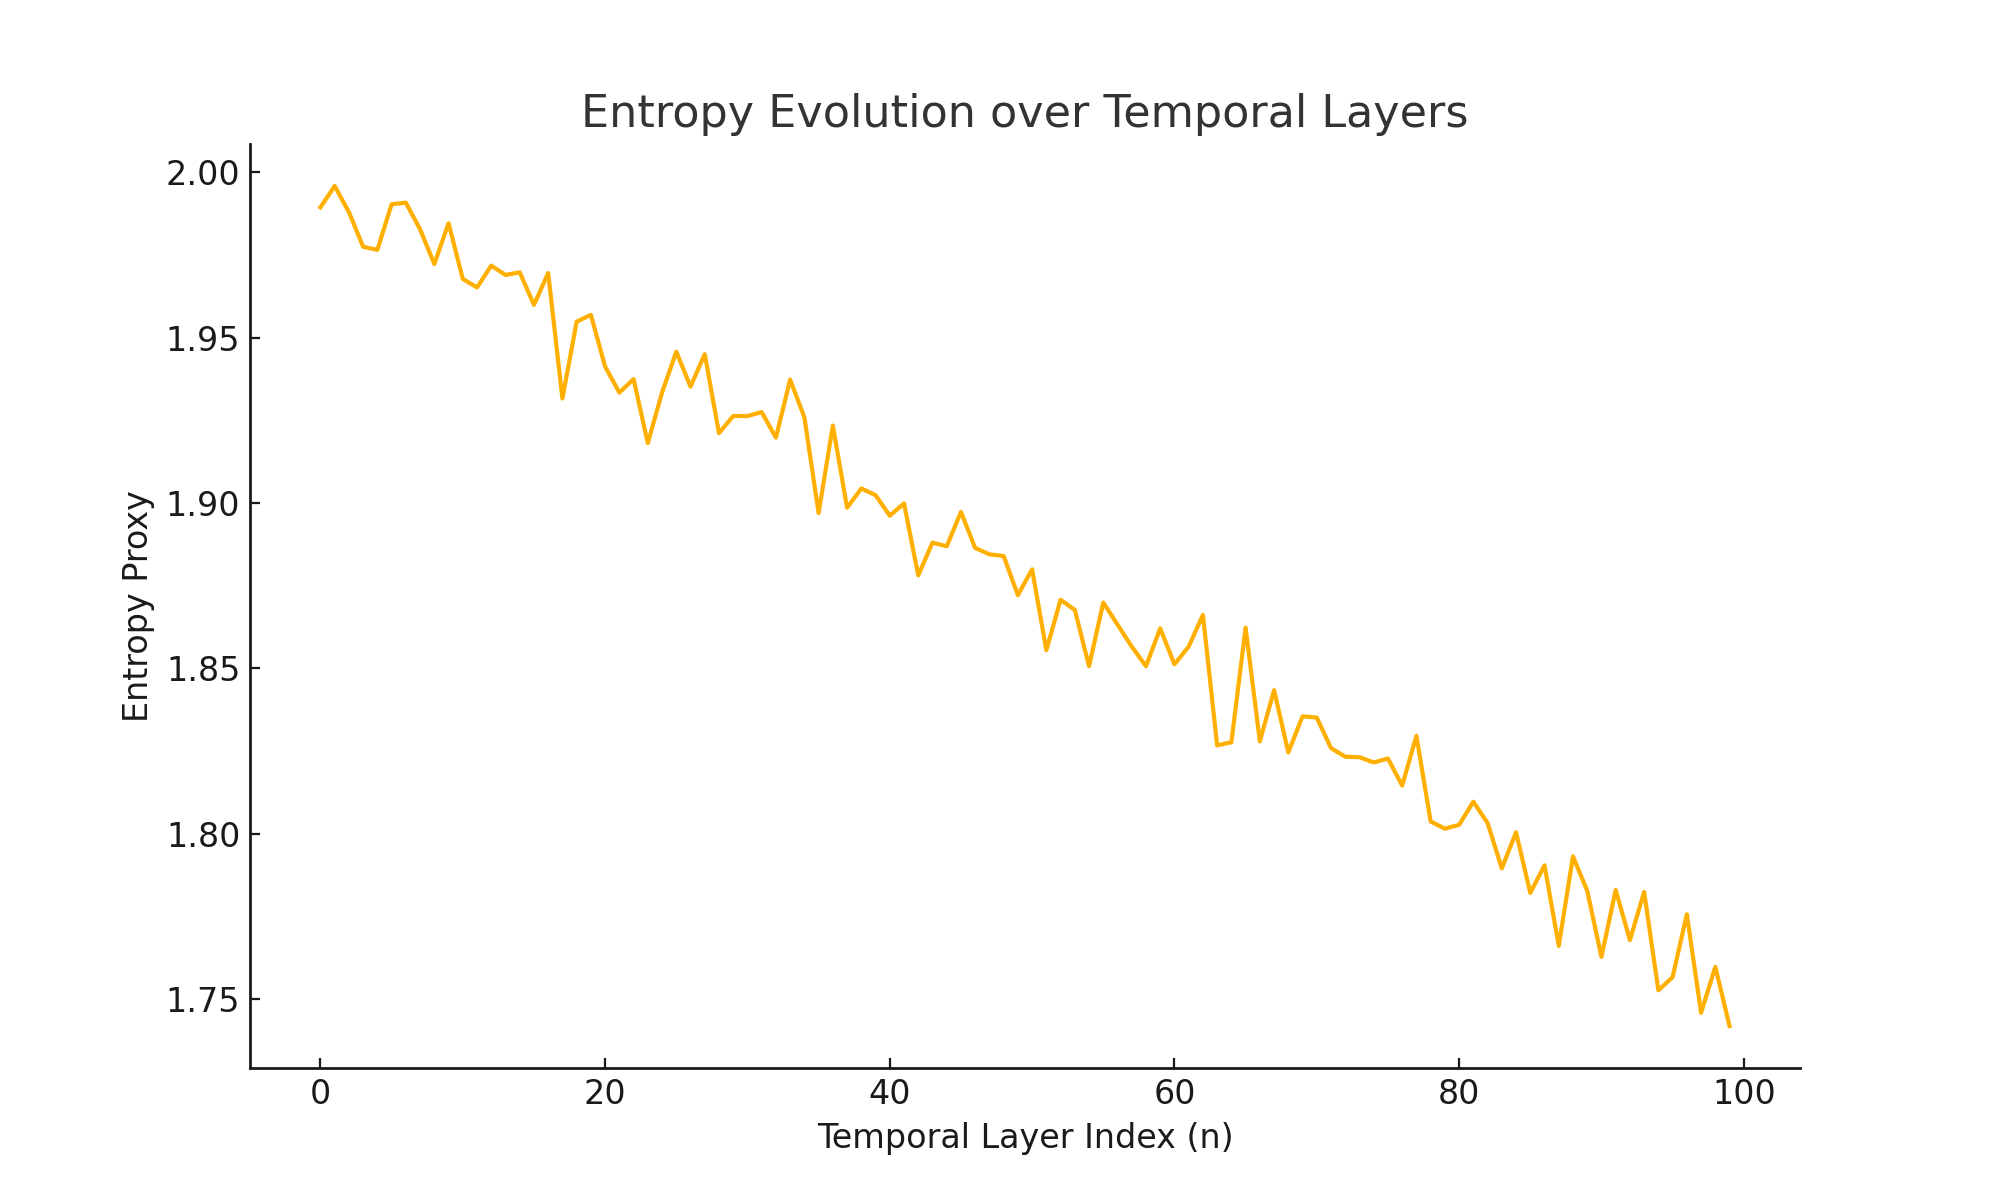
\includegraphics[width=0.9\linewidth]{05_Simulations/entropy_evolution.png}
\caption{Entropy evolution as a function of temporal layer index $n$. The slight decrease simulates entropic decay modulated by stochastic noise.}
\end{figure}

\begin{figure}[h!]
\centering
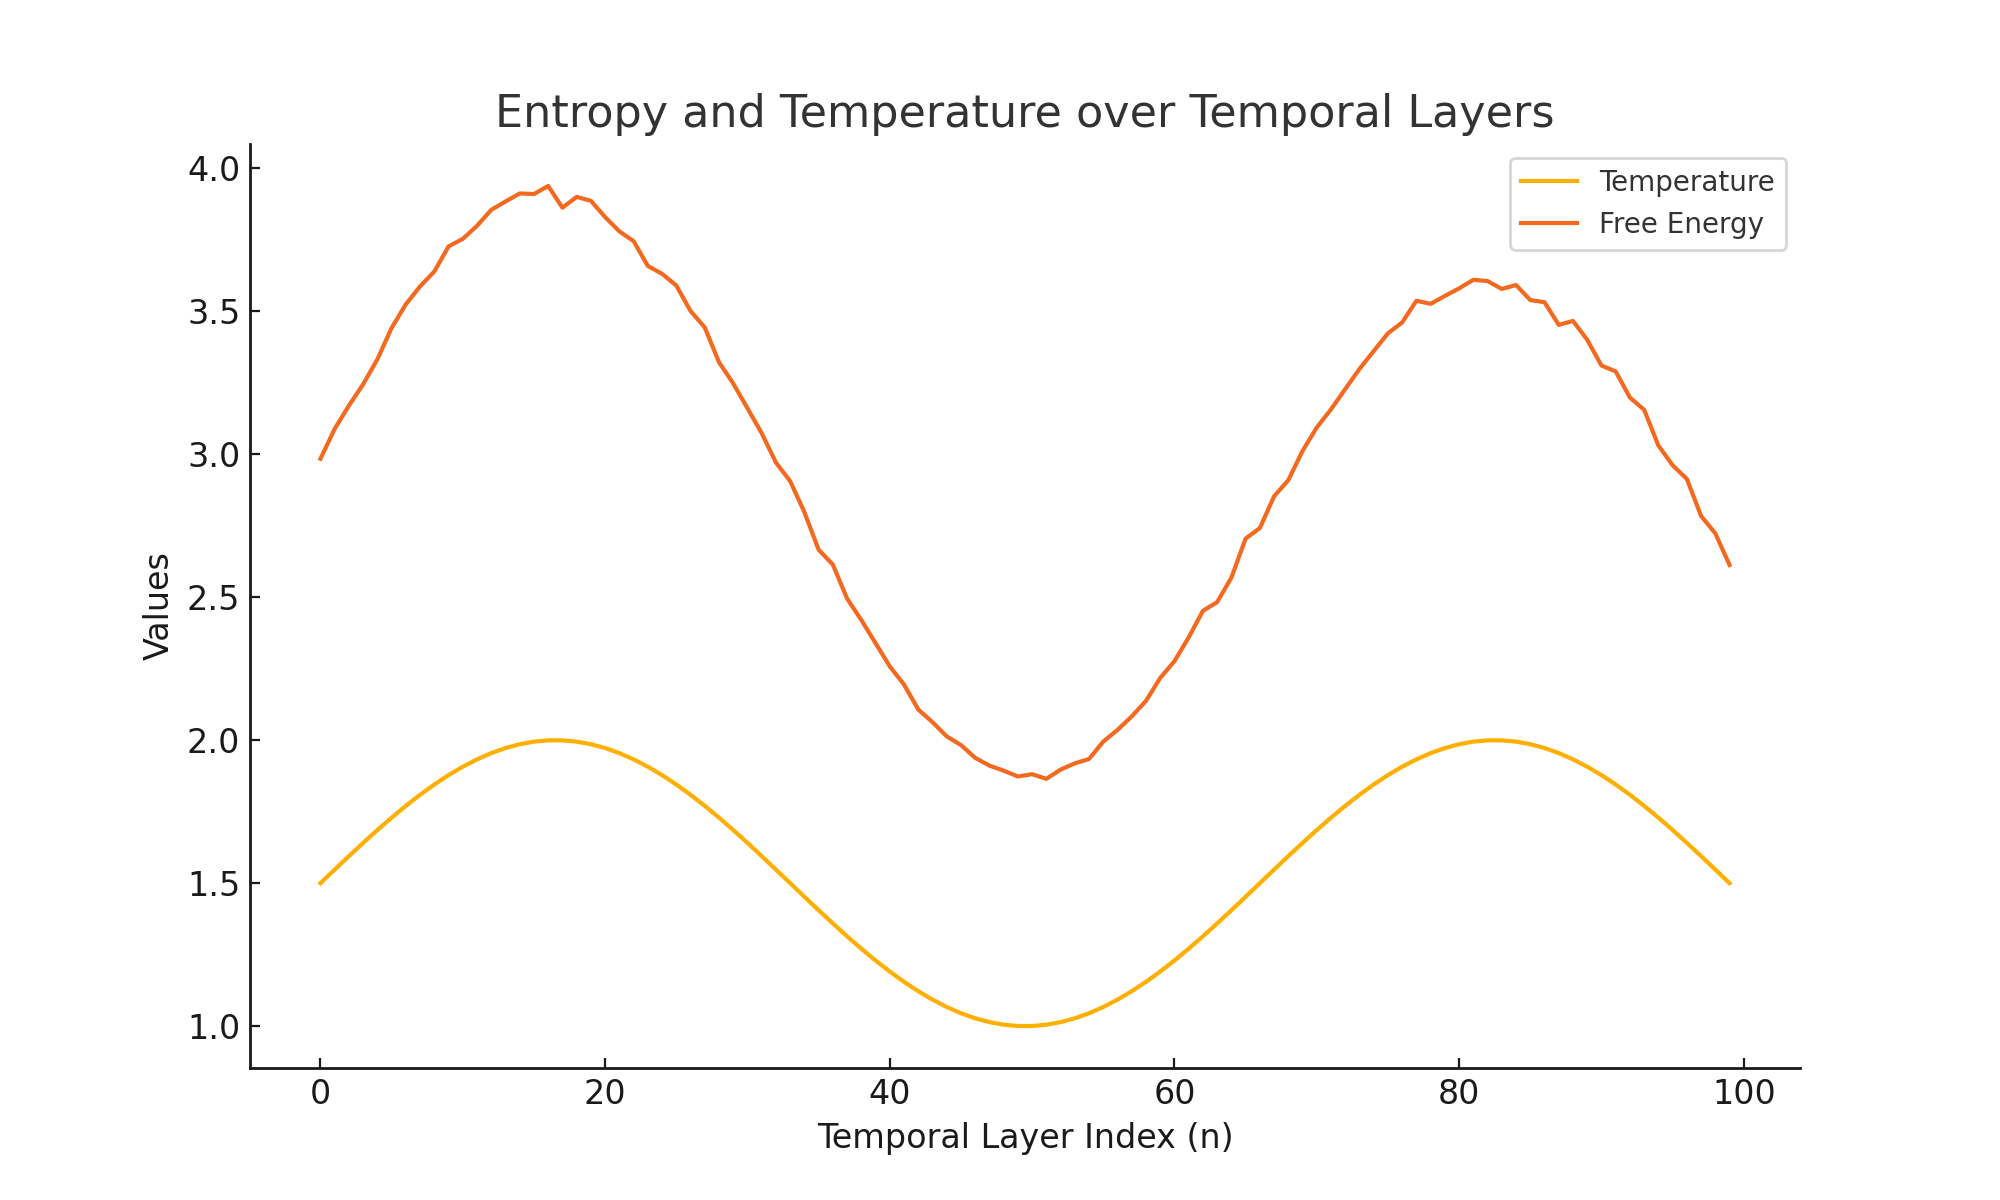
\includegraphics[width=0.9\linewidth]{05_Simulations/temp_free_energy.png}
\caption{Comparison of simulated temperature and free energy over time. Fluctuations are synthetic but reflect thermodynamic oscillations.}
\end{figure}

\begin{figure}[h!]
\centering
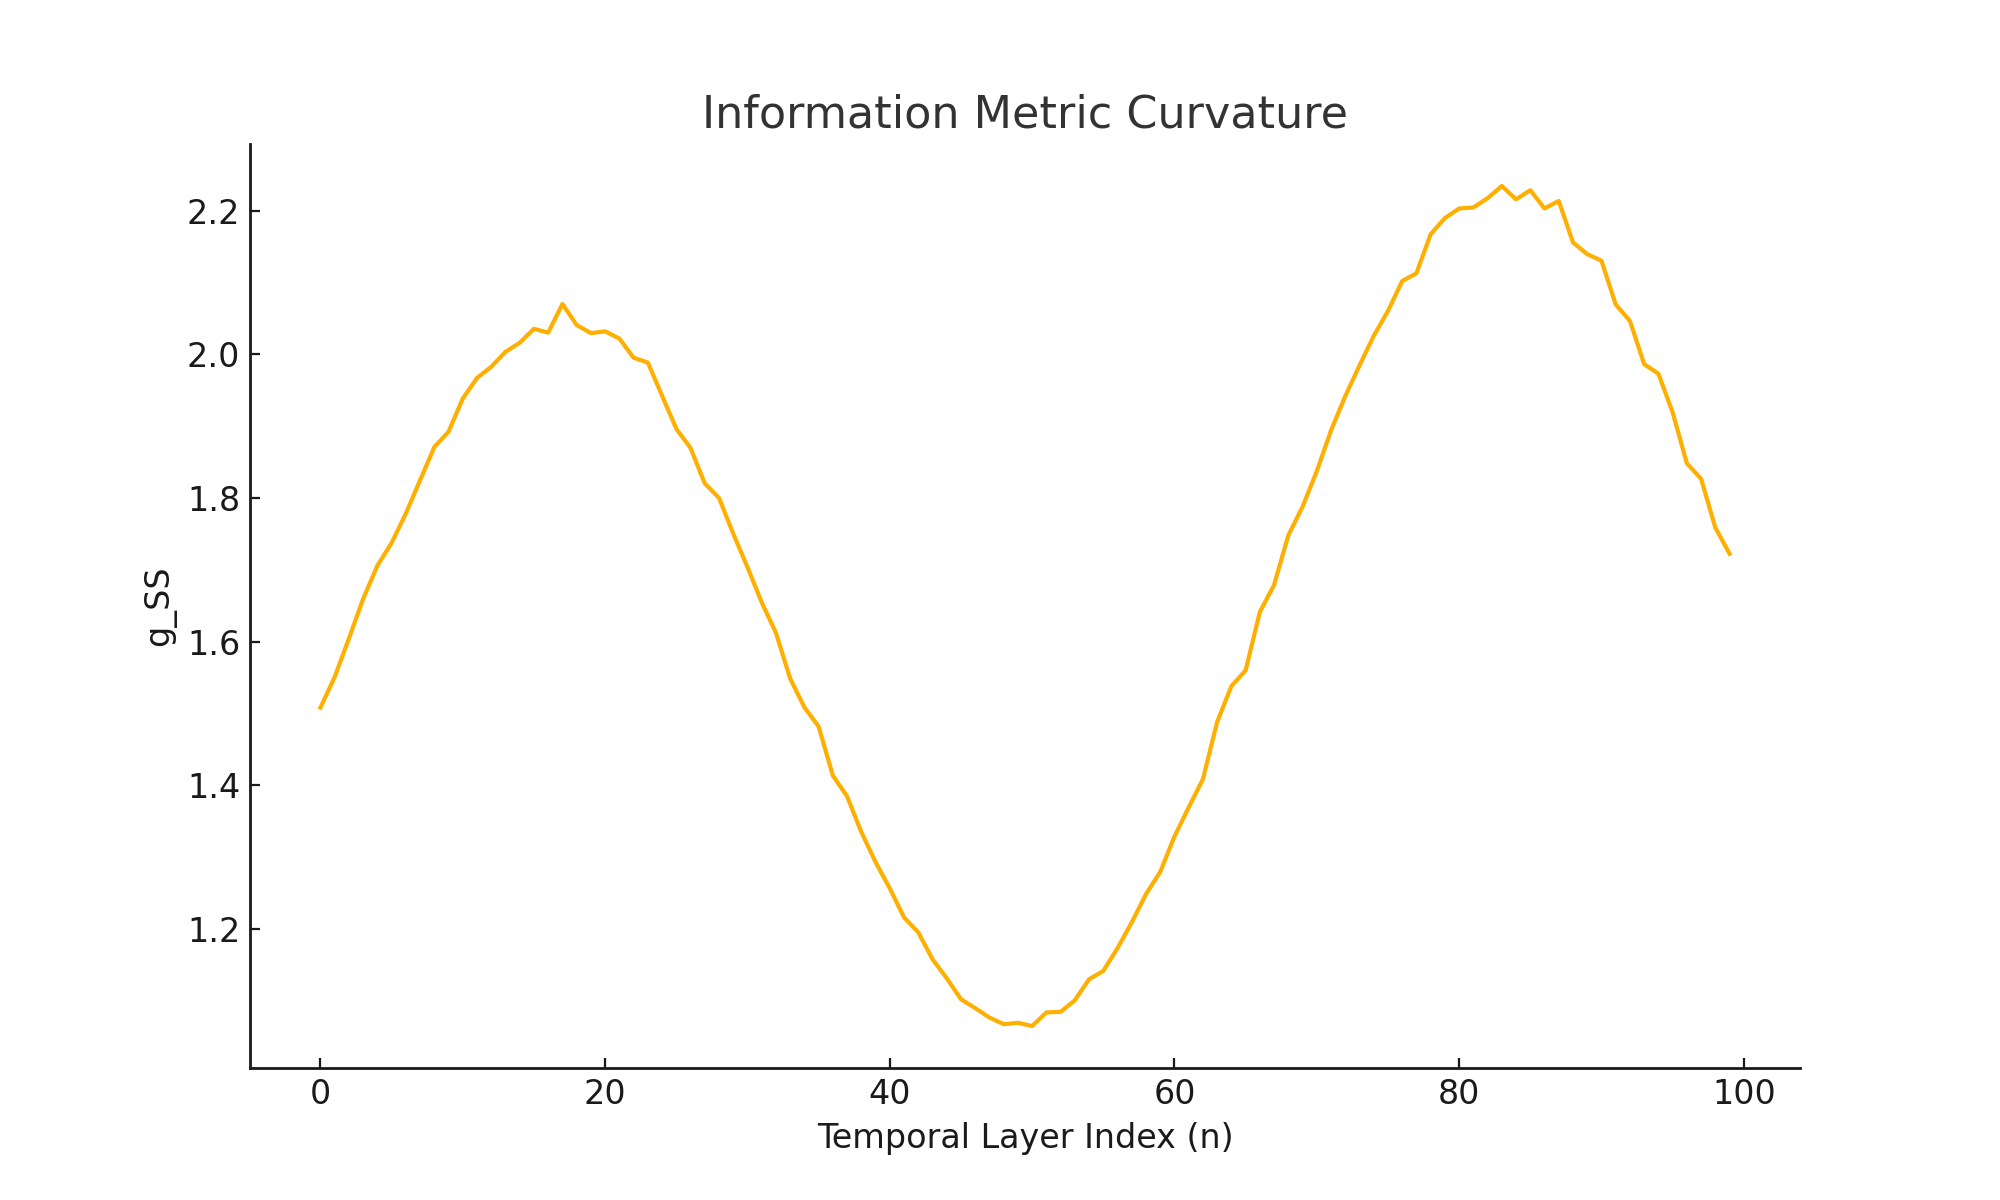
\includegraphics[width=0.9\linewidth]{05_Simulations/info_metric_curvature.png}
\caption{Information metric curvature $g_{SS}$ derived from synthetic entropy and temperature series.}
\end{figure}
